\section{The Project}
\label{sec:the_project}
Automatic content categorization is a process where the text is categorized to the most describing category or categories from a set of desirable categories. There are various ways of performing automatic content categorization. This project focuses on categorizing text based on which keywords occur in the text and these keywords' categories. 

\begin{figure}[h]
\centering
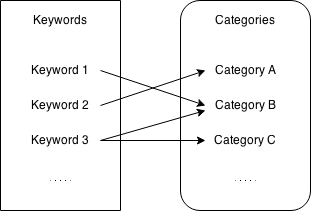
\includegraphics[width=0.65\textwidth]{Chapters/Introduction/keywordstocategories}
\caption{Illustration of the mapping between keywords and categories.}
\label{fig:keywordstocategories}
\end{figure}


Creating this automatic content categorization consists of three main steps. 
\begin{enumerate}
\item Create a list of keywords and a set of desirable categories for the categorization process. For this project, titles of Wikipedia articles are chosen as keywords, and the set of desirable categories is based on the taxonomy from  \emph{Interactive Advertising Bureau} (IAB). 
%The Wikipedia article titles need be processed before they can be used as keywords and some changes might be necessary to create a 
Both Wikipedia article titles and IAB's taxonomy need to be processed before they are suitable as keywords and category set. 
\item Create a mapping between the keywords and the categories (see figure \ref{fig:keywordstocategories}). This step takes advantage of the underlying structure of Wikipedia to determine the meaning of the Wikipedia articles, so that the keywords map to the category or categories that best describe their content.
\item Determine the category of any given text. Figure \ref{fig:categorizetext} shows this process, where all keywords are extracted from the given text and the text's category is determined from the keywords' categories. There are different ways of determining the category of a text. The extraction process could be exact matches of the keywords as they appear in our dictionary or by matching lemmas\footnote{Lemma is defined as the canonical form of a word \cite[][p. 30]{iirbook}.} where all inflections of words are considered equal. It is also possible to let the classifier determine the text's category based on different features; we could for instance count occurrences of all  keywords leading to a category, or only count occurrences of unique keywords. The software for finding keywords in a text is provided by Cxense and is described in detail in section \ref{sec:cxense}.
\end{enumerate}

\subsubsection{Why choose a dictionary-based classifier?}
%Our main motivation for choosing 
We chose a dictionary-based classifier because it is easy to understand for non-technical users. The users of our project are people without any specific knowledge of categorization or computer science. The classifier uses categories written in natural language and gives output the users can understand without help from developers. It is also based on a dictionary, which is a familiar concept that might make it easier to understand the classification process. Another advantage with a dictionary is that it is easy to edit for users, which means that they can personalize the dictionary to fit their preferences by adding/removing entries. 

%, which makes it possible for users to remove or add entries to the dictionary. The categories are also written in natural language, which gives output the users can understand without help from developers. 

\subsubsection{Why use Wikipedia?}
We chose to use Wikipedia titles for our classifier, for 3 main reasons.
\begin{enumerate}
\item Wikipedia is the largest online encyclopedia and is maintained by volunteers from all over the world.
\item Wikipedia contains a useful category structure where all articles are placed within categories descriptive of their content, and the categories form a structure which represents relations between the categories. 
\item Wikipedia titles are words or phrases which are good keywords since they are found within other articles. 
\end{enumerate}


\subsubsection{Access to the results}
All results are based on Wikipedia, downloaded the 22nd of January 2015 from \enwikidatabasedumps. Several programs were made for this project, and they can be found at \ingridthesis.


\begin{comment}
We chose Wikipedia titles for our classifier because it is the largest online encyclopedia. Wikipedia is edited and maintained by volunteers from all over the world, and it covers various topics within different fields.  Another advantage with Wikipedia is  its category structure. All Wikipedia articles are placed within categories descriptive of their content, and the categories form a structure for which represents the relations between the categories. 

we can choose the category that occur most times, 
based on the keywords' occurrences. 
The software for extracting keywords in this project is provided by Cxense, where we 
different inflected forms of a word are grouped together
and the text's category is determined from the keywords' categories. It is common to use lemmatizations when extracting the keywords

The category or categories of the input text can be determined in different ways, for instance finding the  
One way is to count all occurrences of all 
It is also essential to use some technique for finding keywords in the text, and this project has used software from Cxense for this step. 
Example of a categorization could be the simple collection of the two texts: $t_{1}$ = \emph{Zlatan and Messi play soccer} and $t_{2}$ = \emph{The sun in yellow}.  \emph{soccer}, \emph{Messi} and \emph{Zlatan} are keywords mapping to the category \emph{Sports/soccer}
As example should an article which contains the words \emph{soccer}, \emph{Messi} and \emph{Zlatan} should probably be categorized as \emph{Sports/Soccer} if these are available keywords mapped to this category.  

\end{comment}
%nderstanding text is important for 
%utomatic content categorization is useful for determining the meaning of a text which is useful in many settings. 
%Given a set of desirable categories it
%To be able to categorize articles, it is 
%Thus our overall goal is defined as creating a classifier that maps keywords from a predefined keyword list and to one or more pre-defined categories. The automatic categorization will include both the creation of the predefined keyword list and the mapping function, which are both essential for categorizing collections of texts based on their content. 

%Creating this automatic content categorization consists of *** steps. the first step is to find all keywords 


\begin{figure}[h]
\centering

\includegraphics[width=\textwidth]{Chapters/Introduction/categorizetext}
\caption{Simplified illustration of the categorization process.}
\label{fig:categorizetext}
\end{figure}

\begin{comment}
\begin{figure}[H]
\centering
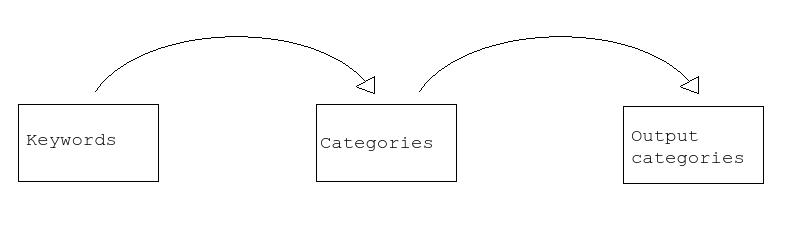
\includegraphics[width=1\textwidth]{Chapters/Introduction/classification_process.jpeg}
\caption{A simplified illustration of the categorization process.}
\label{fig:classification_process}
\end{figure}
\end{comment}
%This classifier will be used as part of an automatic categorization process. 
%Our overall goal is therefore to make an automatic categorization that have a predefined keyword list and start by creating a mapping from each keyword to a category from another predefined list. Where the category of a text can be defined from the keywords found in the text. 

\section{An Overview of Challenges}
We encountered various challenges within different fields while working on this project. Some of the challenges were solved better than others. This section gives a short introduction to some of the most advanced challenges encountered that were more time consuming than the rest.

\subsubsection{Representing the structure}
The structure of Wikipedia is found in multiple files containing lots of information needed for the process of setting up the encyclopedia. The underlying structure is quite complex and is poorly documented from a developer's point of view. The first challenge encountered was deciding which information we needed for our task and where it was found, i.e., which files. Another challenge was to determine how to represent  information and to find suitable structures. 



\begin{comment}
The main challenges encountered had to do with Wikipedia, mainly because the encyclopedia is maintained by thousands of volunteers and is poorly documented from a developer's point of view. The structure of Wikipedia is complex and the size makes it hard to check if the results found are correct. 

\end{comment}

%which also leads to a complicated and complex structure. 

\subsubsection{Encoding and character normalization}
Wikipedia is available in multiple languages and is written by volunteers from all over the world. This makes Wikipedia a multilingual encyclopedia with knowledge available from everywhere since it is possible for experts from various fields and from different parts of the world to contribute with knowledge. There are both advantages and disadvantages with a multilingual encyclopedia. One of the disadvantages is that users might write with different encoding (e.g., \emph{utf8}, \emph{ascii} or \emph{unicode}) because they use different keyboards and different languages. Problems occur when going through all the names of Wikipedia categories and Wikipedia article titles because titles written in different encoding might not be viewed as identical by the computer. 

An example of a category name which lead to encoding trouble is  \emph{Communes in Cara\cb{s}-Severin County}, which is either written with the letter \emph{\cb{s}} (unicode character u\textbackslash 0218) \cite{swithcomma} or \c{s} (unicode character u\textbackslash 015e )  \cite{swithcedilla}. These letters are examples of characters that makes matching of category names difficult, because \emph{Communes in Cara\cb{s}-Severin County} and \emph{Communes in Cara\c{s}-Severin County} will not be equal to the computer even though it is clear to most users that they should be the same. 

This problem was partly solved by changing all category names and article titles to the same encoding by transforming all text to \emph{utf-8}, including escape of \emph{unicode} characters with a python module \emph{Unidecode 0.014.17} which transforms unicode characters to ascii \cite{unidecode}. The results from Unidecode was further converted to utf-8. This solved most of the problem, but some category names did not become equal even though most humans would consider them equal. A total of 10 800 categories was not able to be matched out of 519 822. These categories represent a very small part of all categories  (equivalent to 2.1\%), and were therefore disregarded. 


\subsubsection{Disambiguation}
Antoher problem encountered is disambiguation. Wikipedia contains many titles that could have various meanings (see figure \ref{fig:disambiguation_example}). This means that the titles are ambiguous and leads to the common problem in natural language processing: disambiguation \cite{wiki:disambiguation}. A complete section (\ref{sec:disambiguation}) is dedicated to different solutions to this specific problem. However, our solution was to disregard all ambiguous dictionary entries if they were categorized to different categories.
%others work within in the topic see \ref{sec:disambiguation}

\begin{figure}[h]
\centering
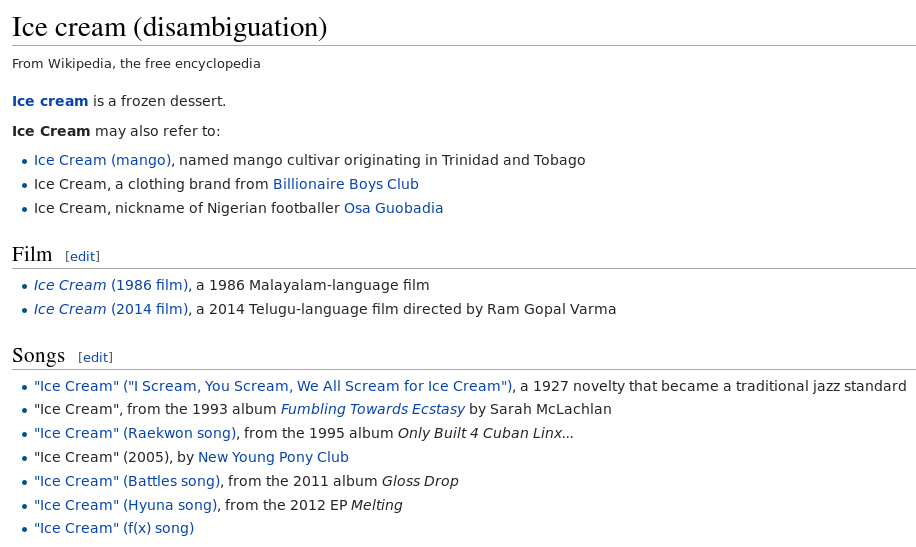
\includegraphics[width=\textwidth]{Chapters/Introduction/Ice_cream_disambiguation}
\caption{Example of disambiguation in Wikipedia.} % \cite{wiki:icecreamdisambiguation}.}
\label{fig:disambiguation_example}
\end{figure}